\chapter{Objetivos de desarrollo sostenible}
\label{chap:OBS}
\Abstract{Análisis comparativo del proyecto frente a los objetivos de desarrollo sostenible. Desde un punto de visto social, ecológico y económico}
El 25 de septiembre de 2015, los líderes mundiales adoptaron un conjunto de objetivos globales para erradicar la pobreza, proteger el planeta y asegurar la prosperidad para todos como parte de una nueva agenda de desarrollo sostenible. Cada objetivo tiene metas específicas que deben alcanzarse en los próximos 15 años.

\begin{figure}[ht]  %OBS
	\centering
	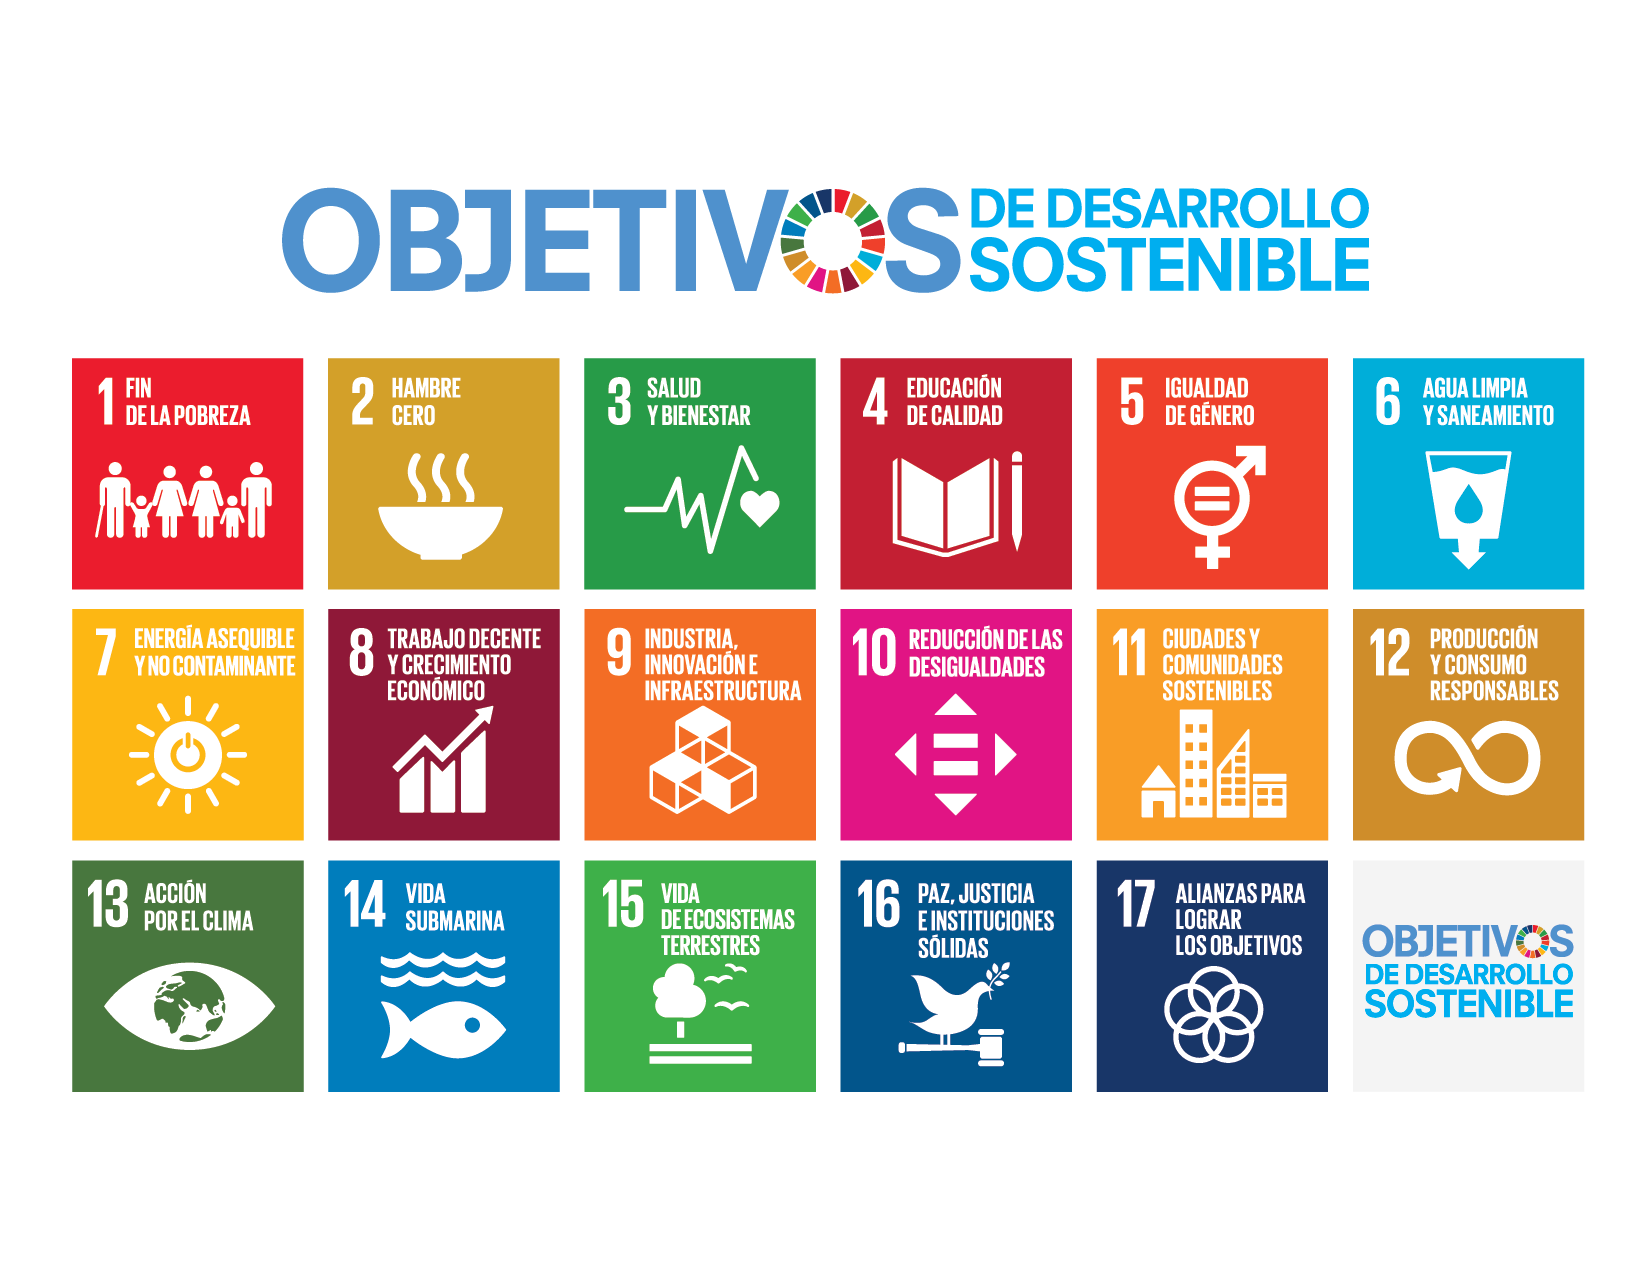
\includegraphics[width=0.8\textwidth]{OBS/esquema.png}
	\vspace{-5pt}
	\caption{Objetivos de desarrollo sostenible aprobados en 2015}
	\label{fig:obs}
\end{figure}

En total se han planteado 17 objetivos para llevar a cabo, este proyecto se enmarca dentro de tres de ellos y a continuación se van a desarrollar de forma individual.

\begin{itemize}
\item Objetivo 8 - Trabajo decente y crecimiento económico: El proceso de automatización de la industria supone la creación de nuevos puestos de trabajo más especializados y con mejores condiciones laborales. Implica un crecimiento de la producción sin un aumento notable de costes y por lo tanto implica un desarrollo económico. Pero par ello es importante controlar este desarrollo y evitar el sobre uso de estas máquinas y con ello el reemplazo del ser humano en el sector industrial.
\item Objetivo 9 - Industria, innovación e infraestructura: Gracias al empleo de las nuevas tecnologías para la automatización de los procesos industriales se ha logrado un crecimiento y desarrollo económico en la industria. Una de las metas de este objetivo es la globalización de estas tecnologías y el facilitar el acceso a estas para los países en vías de desarrollo. Con este proyecto se ha desmostado y creado un sistema reentrenable y usable en el proceso de automatización y esto sin suponer un gran coste de desarrollo. La tecnología desarrollada en este proyecto es de acceso público y modificable para implantar en diferentes sistemas.
\item Objetivo 12 - Producción y consumo responsable: Con la implantación de los robots en la industria no solo se obtiene un incremento en la producción. También, se obtiene una reducción en el número de errores cometidos durante el proceso de fabricación. Esto implica que menos recursos deben de ser usados en la producción. Además, los robots son capaces de desarrollar tareas imposibles para un ser humano y con diferentes materiales. Gracias a sus capacidades, se pueden desarrollar productos más complejos o innovadores centrados en mejorar la sostenibilidad y con un empleo más ecológico de los recursos.
\end{itemize}

Es por todo esto que se considera que este proyecto puede conllevar mejoras para la sociedad a nivel económico, ecológico y social. Siempre y cuando la implantación de estos sistemas se realice correctamente y teniendo en cuenta a la mano de obra humana ya existente. Estos sistemas no deben de reemplazar sino ayudar a este sector.